\section{Durchführung}
\label{sec:Durchführung und Aufbau }
\subsection{Versuchsaufbau}

In dem Versuch wird ein Koaxialer Germanium-Detektor in Zylinder Form verwendet, sein Durchmesser beträgt $\qty{45}{\milli\meter}$ und
seine Länge $\qty{39}{\milli\meter}$. Durch die Eindiffusion von Lithium-Atomen ist die Oberfläche des Detektors n-dotiert, das stellt
eine gute Leitfähigkeit sicher und ermöglicht es, den Pluspol der Sperrspannung anzuschließen.
Im innere des Detektorkristalls befindet sich eine koaxiale Bohrung. Die innere Oberfläche dieser Bohrung ist mit einer 
Goldschicht überzogen, wodurch ein Kontakt zwischen Metall und Halbleiter entsteht, der stark p-dotiert ist. Diese 
intensive p-Dotierung erzeugt eine ausgedehnet Verarmungszone, weil die Akzeptorendichte im Germaniumkristall sehr gering ist.
Eine Aluminium-Schutzhaube umschließt den Detektorkristall vollständig. Sollen Gammaquanten detektiert werden, müssen sie sowohl 
die Aluminium-Schicht, als auch die Li-dotierte Oberfläche durchdringen. Dies führt zu einer minimalen Energiegrenze für nachweisbare
Gammastrahlen. Bei dem verwendeten Detektor liegt diese Grenze zwischen $\qty{40}{\kilo\electronvolt}$ und $\qty{50}{\kilo\electronvolt}$. Um präzise und Messergebnisse zu erhalten, 
sollten für die Bestimmung der Vollenergienachweiswahrscheinlichkeit nur Energien über $\qty{150}{\kilo\electronvolt}$ betrachtet werden.


\begin{figure}
    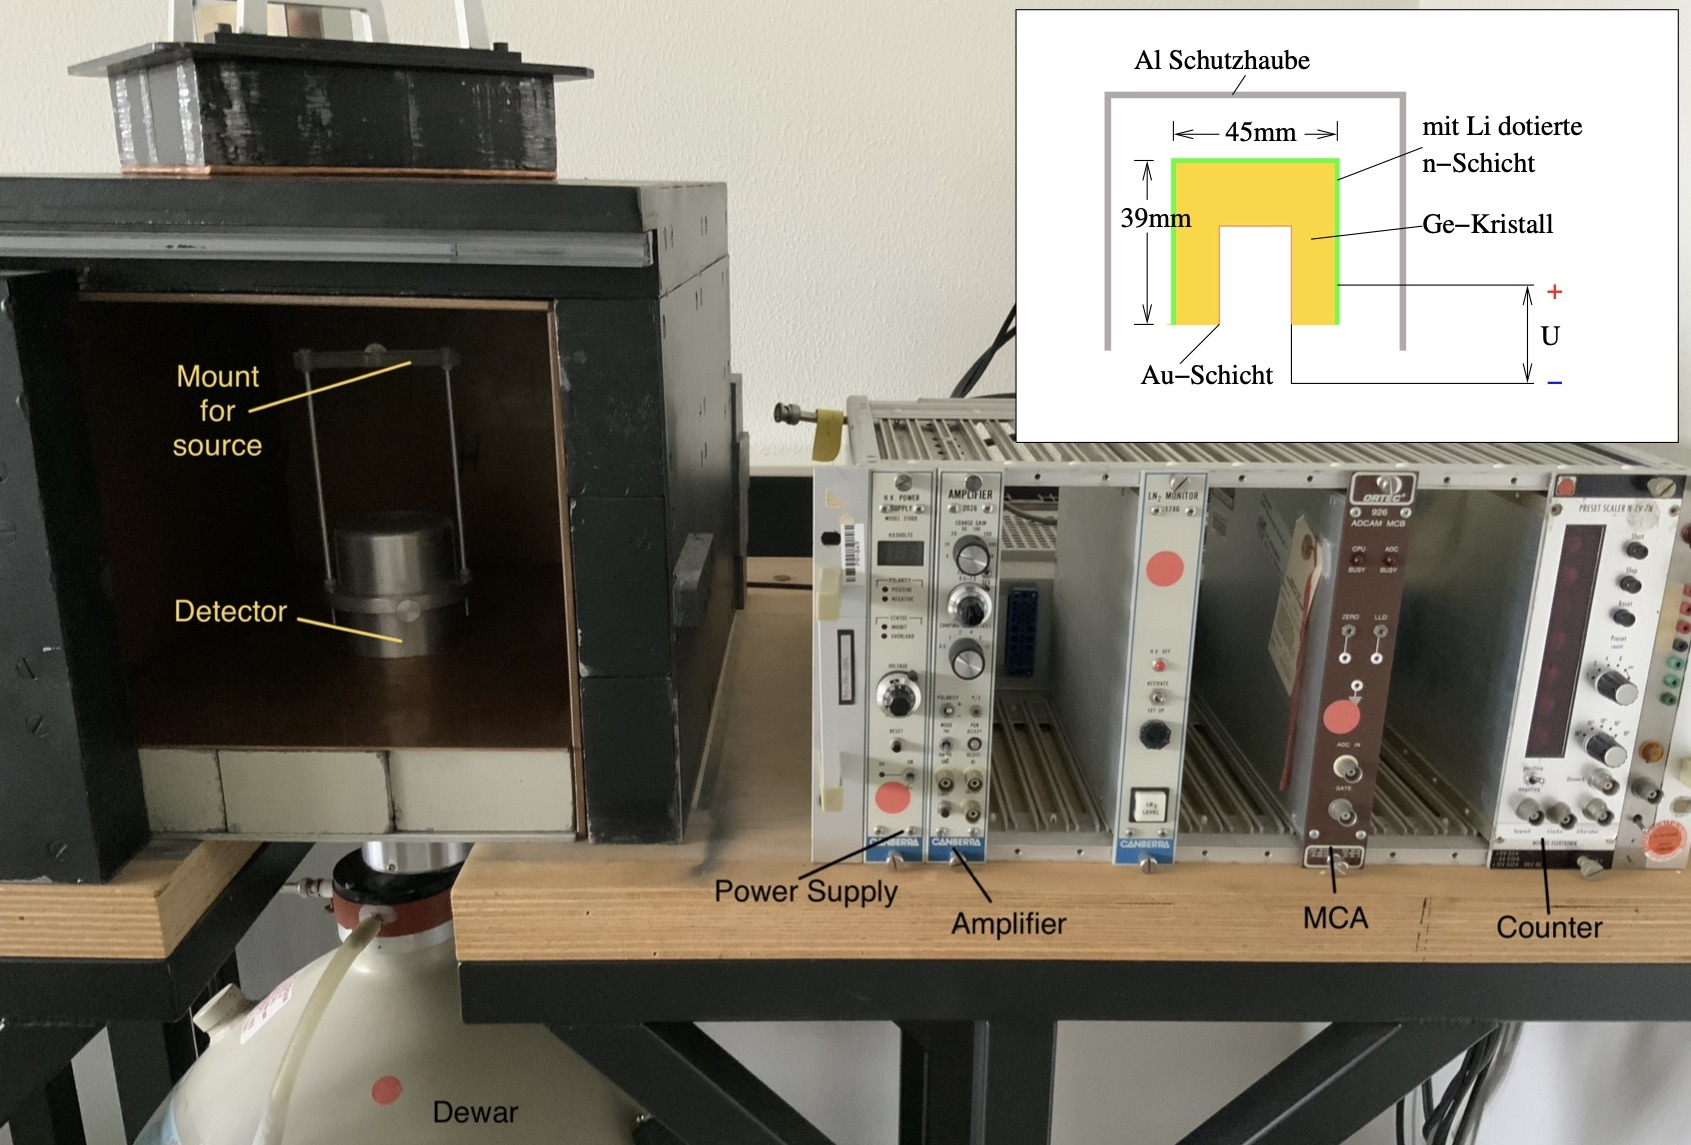
\includegraphics[width=\textwidth]{bilder/aufbau.jpg}
    \caption{Der Aufgebaute Versuch.}
\end{figure}

\cite{aufbau}
\subsection{Durchführung}
Zuerst wird das Spektrum eines $152$-Eu Strahlers erfasst, dessen Emissionsspektrum bekannt ist, um eine Energiekalibration der Apparatur und eine Messung der
Vollenergienachweiswahrscheinlichkeit des Detektors durchzuführen. Dabei sind sowohl die Position der Linien als auch deren Intensität zu bestimmen.
Als nächstes wird das Spektrum eines $^{137}$Cs Strahlers zur Bestimmung von Detektoreigenschaften aufgenommen und zusätzlich die Aktivität der Probe
bestimmt. Eine weiter Aktivitätsmessung wird anschließend für ${133}$-Ba durchgeführt. Der letzte Teil des Versuches besteht dadrin, das Spektrum eines
unbekannten Strahlers aufzuzeichnen und die aktiven Nuklide in der Probe zu identifizieren und zu bennen. Auch hier ist die Aktivität der 
verschiedenen Nuklide zu berechnen.



